\subsubsection{Finite variance}\label{hdassumptionsvariance}

\figref{fig:hdcollisionsvariance} shows the scatter plot for the variance of the
residuals of the total number of collisions. We can clearly identify a trend
here, but the magnitude of the residuals is more than one order lower than the
magnitude of the average predicted response, so we conclude that the assumption
of finite variance still holds. The same considerations can be made for the
total number of messages sent.

\begin{figure}[htb]
	\centering
	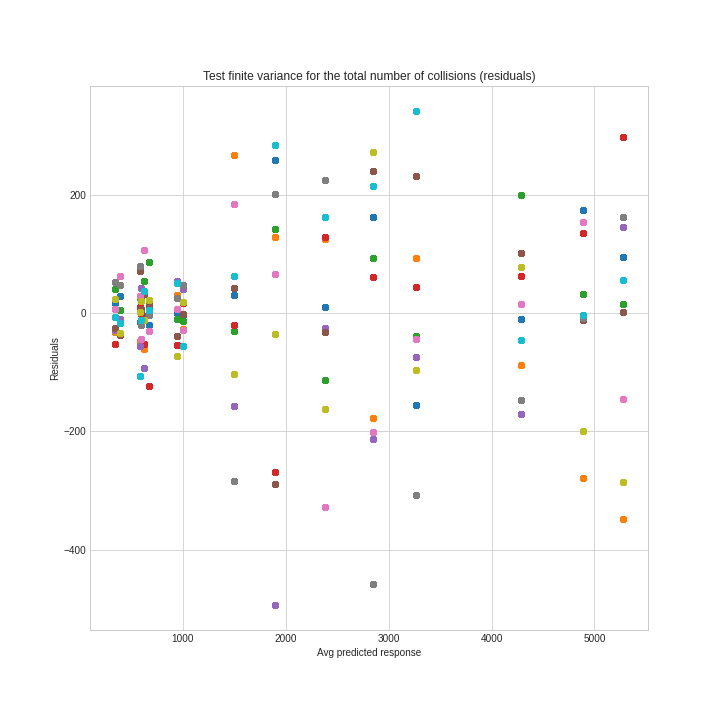
\includegraphics[width=0.75\textwidth]{img/hd/collisions-variance}
	\caption{The scatter plot for the variance of the residuals of the total
	number of collisions shows a trend, but the values on the Y axis are
	much lower than the values on the X
	axis}\label{fig:hdcollisionsvariance}
\end{figure}

\figref{fig:hdtimevariance} shows two scatter plots for the residuals of the
99th percentile of the total broadcast time:
\figref{subfig:hdtimevariancebad}\footnote{From
\code{2kr-assumptions-tests-notransform.ipynb}} shows an increasing trend while
\figref{subfig:hdtimevariancegood} is obtained after performing a logarithmic
transformation of the predicted variable and shows no trend.

\begin{figure}[!ht]
	\centering
	\begin{subfigure}[b]{0.49\textwidth}
		\centering
		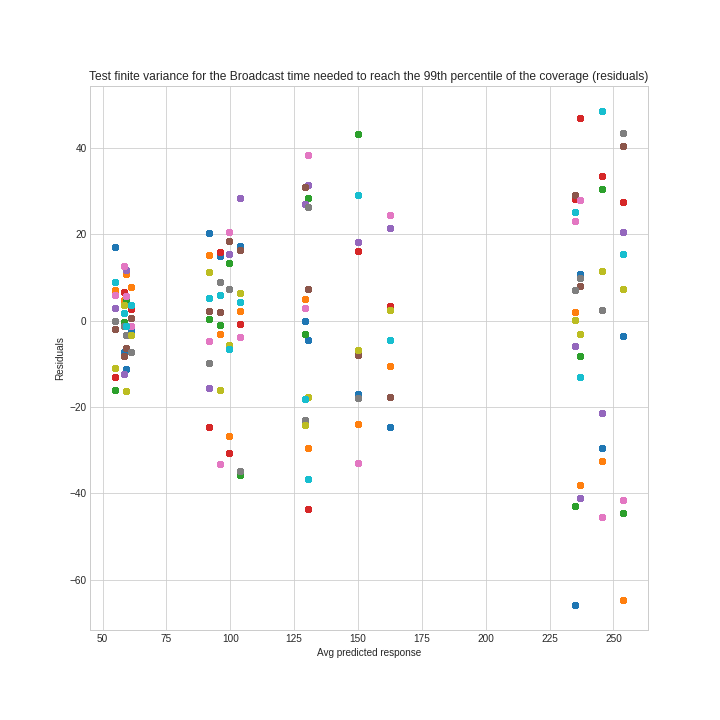
\includegraphics[width=\textwidth]{img/hd/broadcasttime-variance}
		\caption{Clearly a trend is in act
		here}\label{subfig:hdtimevariancebad}
	\end{subfigure}
	\begin{subfigure}[b]{0.49\textwidth}
		\centering
		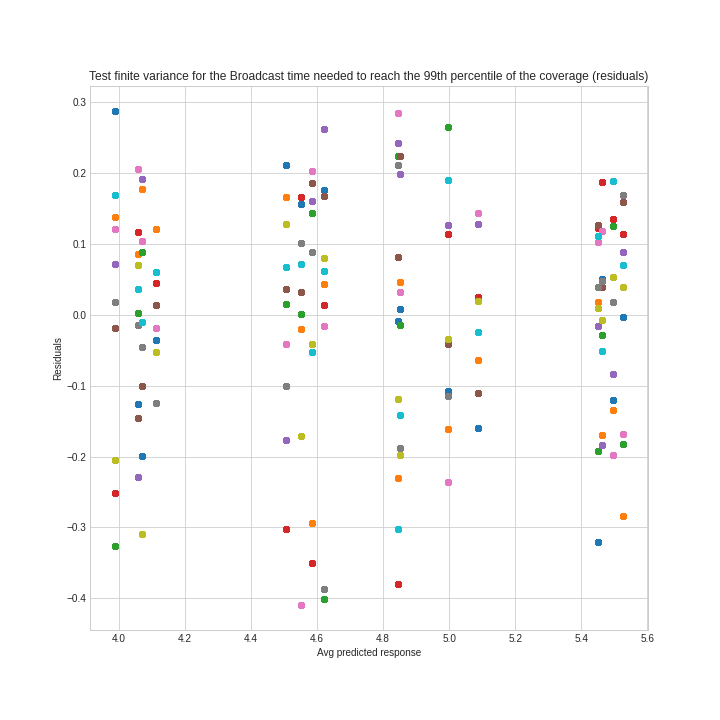
\includegraphics[width=\textwidth]{img/hd/broadcasttime-variance-transform}
		\caption{No trend is shown after the logarithmic
		transformation}\label{subfig:hdtimevariancegood}
	\end{subfigure}
	\caption{Scatter plots of the variance of the residuals of the total
	broadcast time}\label{fig:hdtimevariance}
\end{figure}

So, in order to meet the requirement of finite variance for the residuals of the
total broadcast time, a transformed model is needed: \(y' = \ln(y)\).

